\section{Persistence and completion of the third shooting return}
\label{trc:section}

The preceding section constructed the exact positive-diffusion third
steering equations and proved an initial interval.  This section completes
the finite third shooting return.  The argument uses the strict margins of
the original zero-diffusion stage and uniform continuation of the entire
finite trial family.  It retains both parent responses, all three diffusion
losses, the actual third entry data, and the source pulse normalization.
No coefficient is frozen at its entry value.

Fix once and for all the source profiles and the finite frequency data
selected in \eqref{tge:Y3}.  Extend the already constructed finite systems
to the closed parameter value $d=0$ by setting every displayed diffusion
term to zero.  This extension is an exact member of the same equations.
The number $d_{3,\max}>0$ remains the value in \eqref{tge:d3}.

\subsection{The compact entry graph}

For $0\leq d\leq d_{3,\max}$, let $\mathfrak R_d\subset[0,3]^2$
be the set of pairs $(m_1,m_2)$ whose first and second steering endpoint
vorticities vanish.  The two coordinates refer to the two already
constructed pulse families; no uniqueness is imposed.  Put
\[
 \mathfrak R=\{(d,m_1,m_2):0\leq d\leq d_{3,\max},
                    (m_1,m_2)\in\mathfrak R_d\}.
\]

\begin{lemma}\label{trc:entry-compact}
The set $\mathfrak R$ is compact and every fibre $\mathfrak R_d$ is
nonempty.  The map which starts from a point of $\mathfrak R$, runs the
subsequent holds, the third growth to its actual threshold, and the full
third transition, has a continuous image $\mathcal E$.  Hence the set
$\mathcal E$ of all possible third-steering entry states is compact.  If
$\mathcal E_d$ denotes its fibre at diffusion $d$, then
\begin{equation}\label{trc:entry-semicontinuity}
 \lim_{r\downarrow0}\ 
 \sup_{0\leq d\leq r}\ \sup_{e\in\mathcal E_d}
          \operatorname{dist}(e,\mathcal E_0)=0.
\end{equation}
The actual least-root construction at each $d$ is one point of this graph.
\end{lemma}

\begin{proof}
The first and second return theorems construct their complete trial
families on fixed compact time intervals, with uniform compact bounds for
every $0\leq d\leq d_{3,\max}$.  Their integral equations depend
continuously on the initial data, $d$, and the pulse parameters.  The first
endpoint-vorticity map is continuous on its full parameter box.  The second
endpoint-vorticity map is continuous on the resulting closed first-zero
graph, which is precisely the relative domain on which the second stage
starts from a returned first state.  The nested simultaneous zero set is
therefore closed in the compact box
$[0,d_{3,\max}]\times[0,3]^2$, so it is compact.  Nonemptiness of each
fibre is the first- and second-return existence result, including its
$d=0$ specialization.

After a return, the holding equations are ordinary differential equations
on the proved compact domain.  The third-growth stopping time is the unique
transverse crossing proved in Theorem~\ref{tge:actual_threshold}; the rate
lower bound there keeps the crossing transverse at $d=0$ as well.
Continuous dependence of an ODE flow and the elementary transverse-hitting
time lemma therefore make the holds, the third threshold state, and the
fixed-duration transition continuous on $\mathfrak R$.  Their image
$\mathcal E$ is compact.

To prove \eqref{trc:entry-semicontinuity}, suppose it failed.  Then there
would be $d_n\downarrow0$ and $e_n\in\mathcal E_{d_n}$ whose distance from
$\mathcal E_0$ is bounded below by a positive number.  Compactness of
$\mathfrak R$ supplies a convergent subsequence of the associated root
triples, with limit $(0,m_{1,0},m_{2,0})\in\mathfrak R$.  Continuity of the
entry map sends that subsequence to a point of $\mathcal E_0$, contradicting
the assumed distance.  This proof does not require continuity of the least
root itself.  In particular a jump among zeroes causes no gap.
\end{proof}

At $d=0$, every point of $\mathcal E_0$ is an admissible source entry.
Indeed all damping terms vanish, the coordinate maps in the preceding
sections are exact inverses, and every earlier endpoint zero obeys the same
source endpoint estimates whether or not it is the least zero.  Thus the
source's later-stage comparison applies to every element of
$\mathcal E_0$, not only to one chosen root history.

\subsection{A nonsingular pair coordinate retaining diffusion}

For a third-steering entry $e\in\mathcal E_d$, keep its actual numbers
$P_{3,1},\sigma_2,K_3,\chi_1,s$ and define
\begin{equation}\label{trc:pair-coordinates}
 p=-\frac{\Theta_3}{P_{3,1}},\qquad
 o=-\frac{\sigma_2\Omega_3}{K_3P_{3,1}},\qquad
 \mathcal K=\frac{N_3}{\sigma_2^2\sin s\,R}.
\end{equation}
Then $p(0)=1$ and $o(0)=\chi_1v_1$.  Direct substitution in
\eqref{tr:physical_pair}, with $\tau=\Gamma(t-t_1)$, gives the exact system
\begin{equation}\label{trc:pair-system}
 p'=\mathcal K o-\delta_3Rp,\qquad
 o'=\frac{Z_m}{\sin s}p-\delta_3Ro,qquad
 \delta_3=\frac{dK_3^2}{\Gamma}.
\end{equation}
No division by $\Theta_3$ occurs in this system.  On the open set $p>0$,
\begin{equation}\label{trc:quotient-map}
 v=\frac{o}{\chi_1p},\qquad k=\chi_1\mathcal K,
\end{equation}
and differentiating gives, without discarding the common diffusion,
\begin{equation}\label{trc:quotient-check}
 v'=\frac{Z_m}{\chi_1\sin s}-kv^2,\qquad
 (\log p)'=kv-\delta_3R.
\end{equation}
These are exactly \eqref{tr:quotient}.  The first identity records the
cancellation of equal newest-layer damping in the quotient; the second
retains its complete contribution to the temperature gain.

Combine \eqref{tr:scaled} with \eqref{trc:pair-system}.  Algebraic
quantities $D,x,y,R,Y,\zeta_1,\zeta_2,\zeta_3,N_2,N_3$ retain the definitions
in \eqref{tr:coordinates}--\eqref{tr:inverse}.  The resulting dimensionless
state can be written
\[
 X=(h,g,E,F,\omega,V,p,o).
\]
Together with the constant entry parameters, it has a smooth vector field
on the open component domain where the three phase second components,
$D,R,Y,N_2,N_3$, and the control denominators are positive.  The pulse
$Z_m$ is smooth at both joins.  The vector field is jointly continuous in
$d,e,m,\tau$ and locally Lipschitz in $X$, uniformly on compact subsets of
that domain.

\subsection{Strict zero-diffusion margins}

Let $T=1+L^{-1}$ and let $F_0(e,m)$ be the source quotient $v(T)$ at
$d=0$.  Write $W_0(e,m)=\Omega_2(T)/\sigma_2$ and
$G_0(e,m)=\log p(T)$.  At a zero of $F_0$, set
\[
 \mathcal C_0(e,m)=
 \frac{2\dot\alpha(T)+\Omega_1(T)+\Omega_2(T)}{\sigma_2}.
\]
The third term $\Omega_3(T)$ is zero there.  The constant $c_W>0$ is the
fixed source constant in (3.14) and (3.19).

\begin{lemma}\label{trc:source-margins}
For every $e\in\mathcal E_0$, the complete source trial family exists on
$[0,T]$ in one common compact subset of the smooth component domain, and
$p>0$.  Its endpoint margins are
\begin{equation}\label{trc:endpoint-margins}
 F_0(e,0)\geq\frac18,
 \qquad F_0(e,3)\leq-1.
\end{equation}
The zero set
\[
 \mathcal Z_0=\{(e,m)\in\mathcal E_0\times[0,3]:F_0(e,m)=0\}
\]
is compact, and every $(e,m)\in\mathcal Z_0$ satisfies
\begin{equation}\label{trc:root-margins}
 W_0(e,m)\geq\frac1{12},\qquad
 G_0(e,m)\geq\frac16,
 \qquad \mathcal C_0(e,m)\geq c_W.
\end{equation}
\end{lemma}

\begin{proof}
At $d=0$ the complete finite equations reduce exactly to the source
controlled system.  The frequency choices remain in the same source
family, and the schedule choice places the model error
$\delta_{\rm mdl}$ inside Lemma~3.9 of the source.  In that lemma the
comparison constant $C_{\rm cmp}$ and the chosen tolerance obey
$C_{\rm cmp}\delta_{\rm mdl}\leq1/4$.

On the first steering part, source (3.40) at $\tau=1$ gives
\[
 v(1)\geq\frac{1-C_{\rm cmp}\delta_{\rm mdl}}2\geq\frac38,
 \qquad v(1)<\bar v=2.
\]
Source (3.44) then gives
\[
 v(T;0)\geq v(1)-C_{\rm cmp}\delta_{\rm mdl}\geq\frac18,
 \qquad
 v(T;3)\leq v(1)-3<-1,
\]
which proves \eqref{trc:endpoint-margins}; weakening the last strict
inequality to the displayed non-strict bound is harmless.

For every endpoint zero, source (3.45) gives
\[
 W_0(T)\geq\frac13-C_{\rm cmp}\delta_{\rm mdl}\geq\frac1{12}.
\]
Source (3.46), including $I_0\geq2/9$, gives
\[
 G_0=\int_0^Tkv\,d\tau
 \geq(1-C_{\rm cmp}\delta_{\rm mdl})I_0
 \geq\frac34\frac29=\frac16.
\]
At a return the proof of source (3.19) uses this positive preceding-layer
vorticity and the complete older feedback sum to give
$2\dot\alpha+\Omega_1+\Omega_2\geq c_W\sigma_2$.
That calculation uses only the endpoint bounds shared by every zero, so it
does not depend on which zero is selected.

Source Section~3.7.6 first constructs the geometry for every trial in a
common compact subset of its smooth domain.  It then solves the newest
linear pair and excludes a temperature zero by its bounded quotient.
Consequently $p>0$ for every trial.  Compactness of
$\mathcal E_0\times[0,3]\times[0,T]$ and continuous dependence make the
union of these trajectories compact and give a positive minimum for $p$.
Continuity of $F_0$ makes $\mathcal Z_0$ closed in a compact set, proving
its compactness.
\end{proof}

The strict inequalities on $\mathcal Z_0$ also control nearby almost-zero
endpoints.  More precisely, compactness supplies an open neighborhood
$\mathcal U$ of $\mathcal Z_0$ in
$\mathcal E_0\times[0,3]$ on which
\begin{equation}\label{trc:near-root-margins}
 W_0>\frac1{24},\qquad G_0>\frac1{12},
 \qquad \mathcal C_0>\frac{c_W}{2}.
\end{equation}
Because $F_0$ has no zero in the compact complement of $\mathcal U$, the
number
\begin{equation}\label{trc:eta}
 \eta_*=min_{(e,m)\in
  (\mathcal E_0\times[0,3])\setminus\mathcal U}|F_0(e,m)|
\end{equation}
is positive.

\subsection{Uniform continuation and the selected return}

\begin{theorem}\label{trc:third-return}
There is a number
\[
 0<d_{\rm ret}\leq d_{3,\max},
\]
determined by the fixed source profiles, the finite frequency data, and
the already constructed first two return families before a third root is
selected, with the following property.  For every
$0<d\leq d_{\rm ret}$, the entire actual third trial family
$m\in[0,3]$ exists through $\tau=T$.  All original matrices and controls
are smooth, every source phase second component is positive, and
$\Theta_3<0$ on every trial.  Its endpoint quotient obeys
\begin{equation}\label{trc:diffusive-signs}
 v(T;0)\geq\frac1{16},\qquad
 v(T;3)\leq-\frac{15}{16}.
\end{equation}
Hence its endpoint-zero set is a nonempty compact subset of $(0,3)$ and
has a least member $m_{3,*}(d)$.

Every endpoint zero, including this least one, satisfies
\begin{equation}\label{trc:diffusive-root-bounds}
 \frac{\Omega_2(T)}{\sigma_2}\geq\frac1{48},\qquad
 \log\frac{-\Theta_3(T)}{-\Theta_3(0)}\geq\frac1{24},
 \qquad
 \frac{2\dot\alpha(T)+\Omega_1(T)+\Omega_2(T)}{\sigma_2}
       \geq\frac{c_W}{4}.
\end{equation}
At the selected endpoint,
\begin{equation}\label{trc:return-state}
 Z_{m_{3,*}}(T)=0,\qquad \Omega_3(T)=0,
 \qquad \Theta_3(T)<0.
\end{equation}
Thus the actual third return, its positive preceding-layer vorticity, its
positive temperature gain, and its positive origin curl all hold at one
fixed positive physical viscosity and thermal diffusivity.
\end{theorem}

\begin{proof}
Let $\mathscr T_0$ be the union of the inviscid trajectories in
Lemma~\ref{trc:source-margins}.  It is compact and lies in the open smooth
component domain.  Choose a compact neighborhood $\mathscr N$ of
$\mathscr T_0$ still contained in that domain.  Let $p_*>0$ be the minimum
of $p$ on $\mathscr T_0$.  The vector field and its state derivative are
bounded on $\mathscr N$, uniformly in $e\in\mathcal E_0$,
$m\in[0,3]$, and $\tau\in[0,T]$.

We first prove uniform existence and convergence.  If no positive
diffusion interval had this property, there would be $d_n\downarrow0$,
entries $e_n\in\mathcal E_{d_n}$, and trials $m_n\in[0,3]$ whose maximal
solutions either left $\mathscr N$ or failed to reach $T$.  By
Lemma~\ref{trc:entry-compact}, after taking a subsequence,
$e_n\to e_0\in\mathcal E_0$; also $m_n\to m_0\in[0,3]$.
The integral equations and the uniform state-Lipschitz bound give the
usual Gronwall estimate on every common initial interval.  Since the
vector fields and entries converge, the $d_n$ solutions converge uniformly
to the complete inviscid solution from $(e_0,m_0)$.  That solution remains
in the interior of $\mathscr N$ and has $p\geq p_*$.  For large $n$ the
$d_n$ solution therefore cannot be the first one to reach the boundary of
$\mathscr N$ or $p=p_*/2$; the local continuation theorem then extends it
past the alleged endpoint.  This contradiction proves that, for all
sufficiently small positive $d$, every trial exists through $T$, remains
in $\mathscr N$, and has $p\geq p_*/2$.  The same contradiction argument
proves uniform convergence of the complete trial family to
$\mathscr T_0$ as $d\downarrow0$.

The endpoint observables $F=v=o/(\chi_1p)$, $W=V(T)$,
$G=\log p(T)$, and $\mathcal C$ are continuous on this compact family.
Uniform convergence therefore permits one common positive radius in $d$
for which
\begin{align*}
 |F_d(e,m)-F_0(e_0,m)|&<\min\{1/16,\eta_*/2\},\\
 |W_d(e,m)-W_0(e_0,m)|&<1/48,\\
 |G_d(e,m)-G_0(e_0,m)|&<1/24,\\
 |\mathcal C_d(e,m)-\mathcal C_0(e_0,m)|&<c_W/4,
\end{align*}
whenever $e\in\mathcal E_d$ and a nearest inviscid entry $e_0$ is chosen
as in \eqref{trc:entry-semicontinuity}.  Shrink that radius further, if
needed, to retain the already proved positive phase-component and matrix
domains.  Let $\mathscr A$ be the set of radii
$r\in(0,d_{3,\max}]$ for which these four uniform estimates, all
smooth-component inequalities, and $p\geq p_*/2$ hold simultaneously for
every $0\leq d\leq r$.  Define
\begin{equation}\label{trc:dret-definition}
 d_{\rm ret}=\frac12\sup\mathscr A.
\end{equation}
The preceding argument proves that $\mathscr A$ contains a positive
interval, so $0<d_{\rm ret}\leq d_{3,\max}/2$.  Its definition uses only
fixed data and complete trial families, before choosing the third root.

Apply the first observable estimate at $m=0,3$ and use
\eqref{trc:endpoint-margins}.  This gives
\[
 F_d(e,0)\geq\frac18-\frac1{16}=\frac1{16},\qquad
 F_d(e,3)\leq-1+\frac1{16}=-\frac{15}{16},
\]
proving \eqref{trc:diffusive-signs}.  The endpoint map is continuous in
$m$ by its integral equation, so the intermediate value theorem gives a
zero.  Its zero set is closed, excludes both endpoints, and is contained
in the compact interval $[0,3]$; hence it is compact and has a least
element.

If $F_d(e,m)=0$, the first observable estimate gives
$|F_0(e_0,m)|<\eta_*$.  Definition \eqref{trc:eta} forces
$(e_0,m)\in\mathcal U$.  Combining
\eqref{trc:near-root-margins} with the other three observable estimates
proves \eqref{trc:diffusive-root-bounds}.  Finally $p(T)>0$ means
$\Theta_3(T)<0$.  Since $v(T)=0$ and every factor in
\eqref{trc:quotient-map} is finite and nonzero, $o(T)=0$ and therefore
$\Omega_3(T)=0$.  The pulse is supported in the interior of its interval,
so $Z_m(T)=0$.  This proves \eqref{trc:return-state} and all assertions.
\end{proof}

\subsection{Exact holding continuation}

On the selected endpoint, prescribe $Z=0$.  The restriction
\eqref{tr:hold} then gives
\begin{equation}\label{trc:holding}
 \Omega_3(t)=0,\qquad
 \Theta_3(t)=\Theta_3(t_3^b)
 \exp\!\left(-dK_3^2\int_{t_3^b}^{t}R(r)\,dr\right)<0
\end{equation}
for as long as the older system exists.  This proves invariance of the
return submanifold with the full temperature diffusion retained.  The
parents continue according to \eqref{tr:hold}; neither is frozen.  Since
$Z$ is flat at the pulse endpoint and $\Omega_3=0$, repeated
differentiation of the vorticity equation shows that all right-end
derivatives of $\Omega_3$ vanish there.  The join is smooth, while
$\Theta_3$ follows the nonstationary decay in \eqref{trc:holding}.

The proof is finite-stage.  It neither supplies a diffusion interval
uniform in the layer number nor establishes the terminal smooth-force
extension.  Those remain the next separate calculations.

The exact algebra in \eqref{trc:pair-system}--\eqref{trc:quotient-check}
and all rational margins in
\eqref{trc:endpoint-margins}--\eqref{trc:diffusive-root-bounds} are checked
by \path{third_return/checks/third_return_persistence_check.py}.  The compact-family
mechanism and the endpoint implications are displayed in
Figure~\ref{trc:fig:persistence}.

\begin{figure}[htbp]
 \centering
 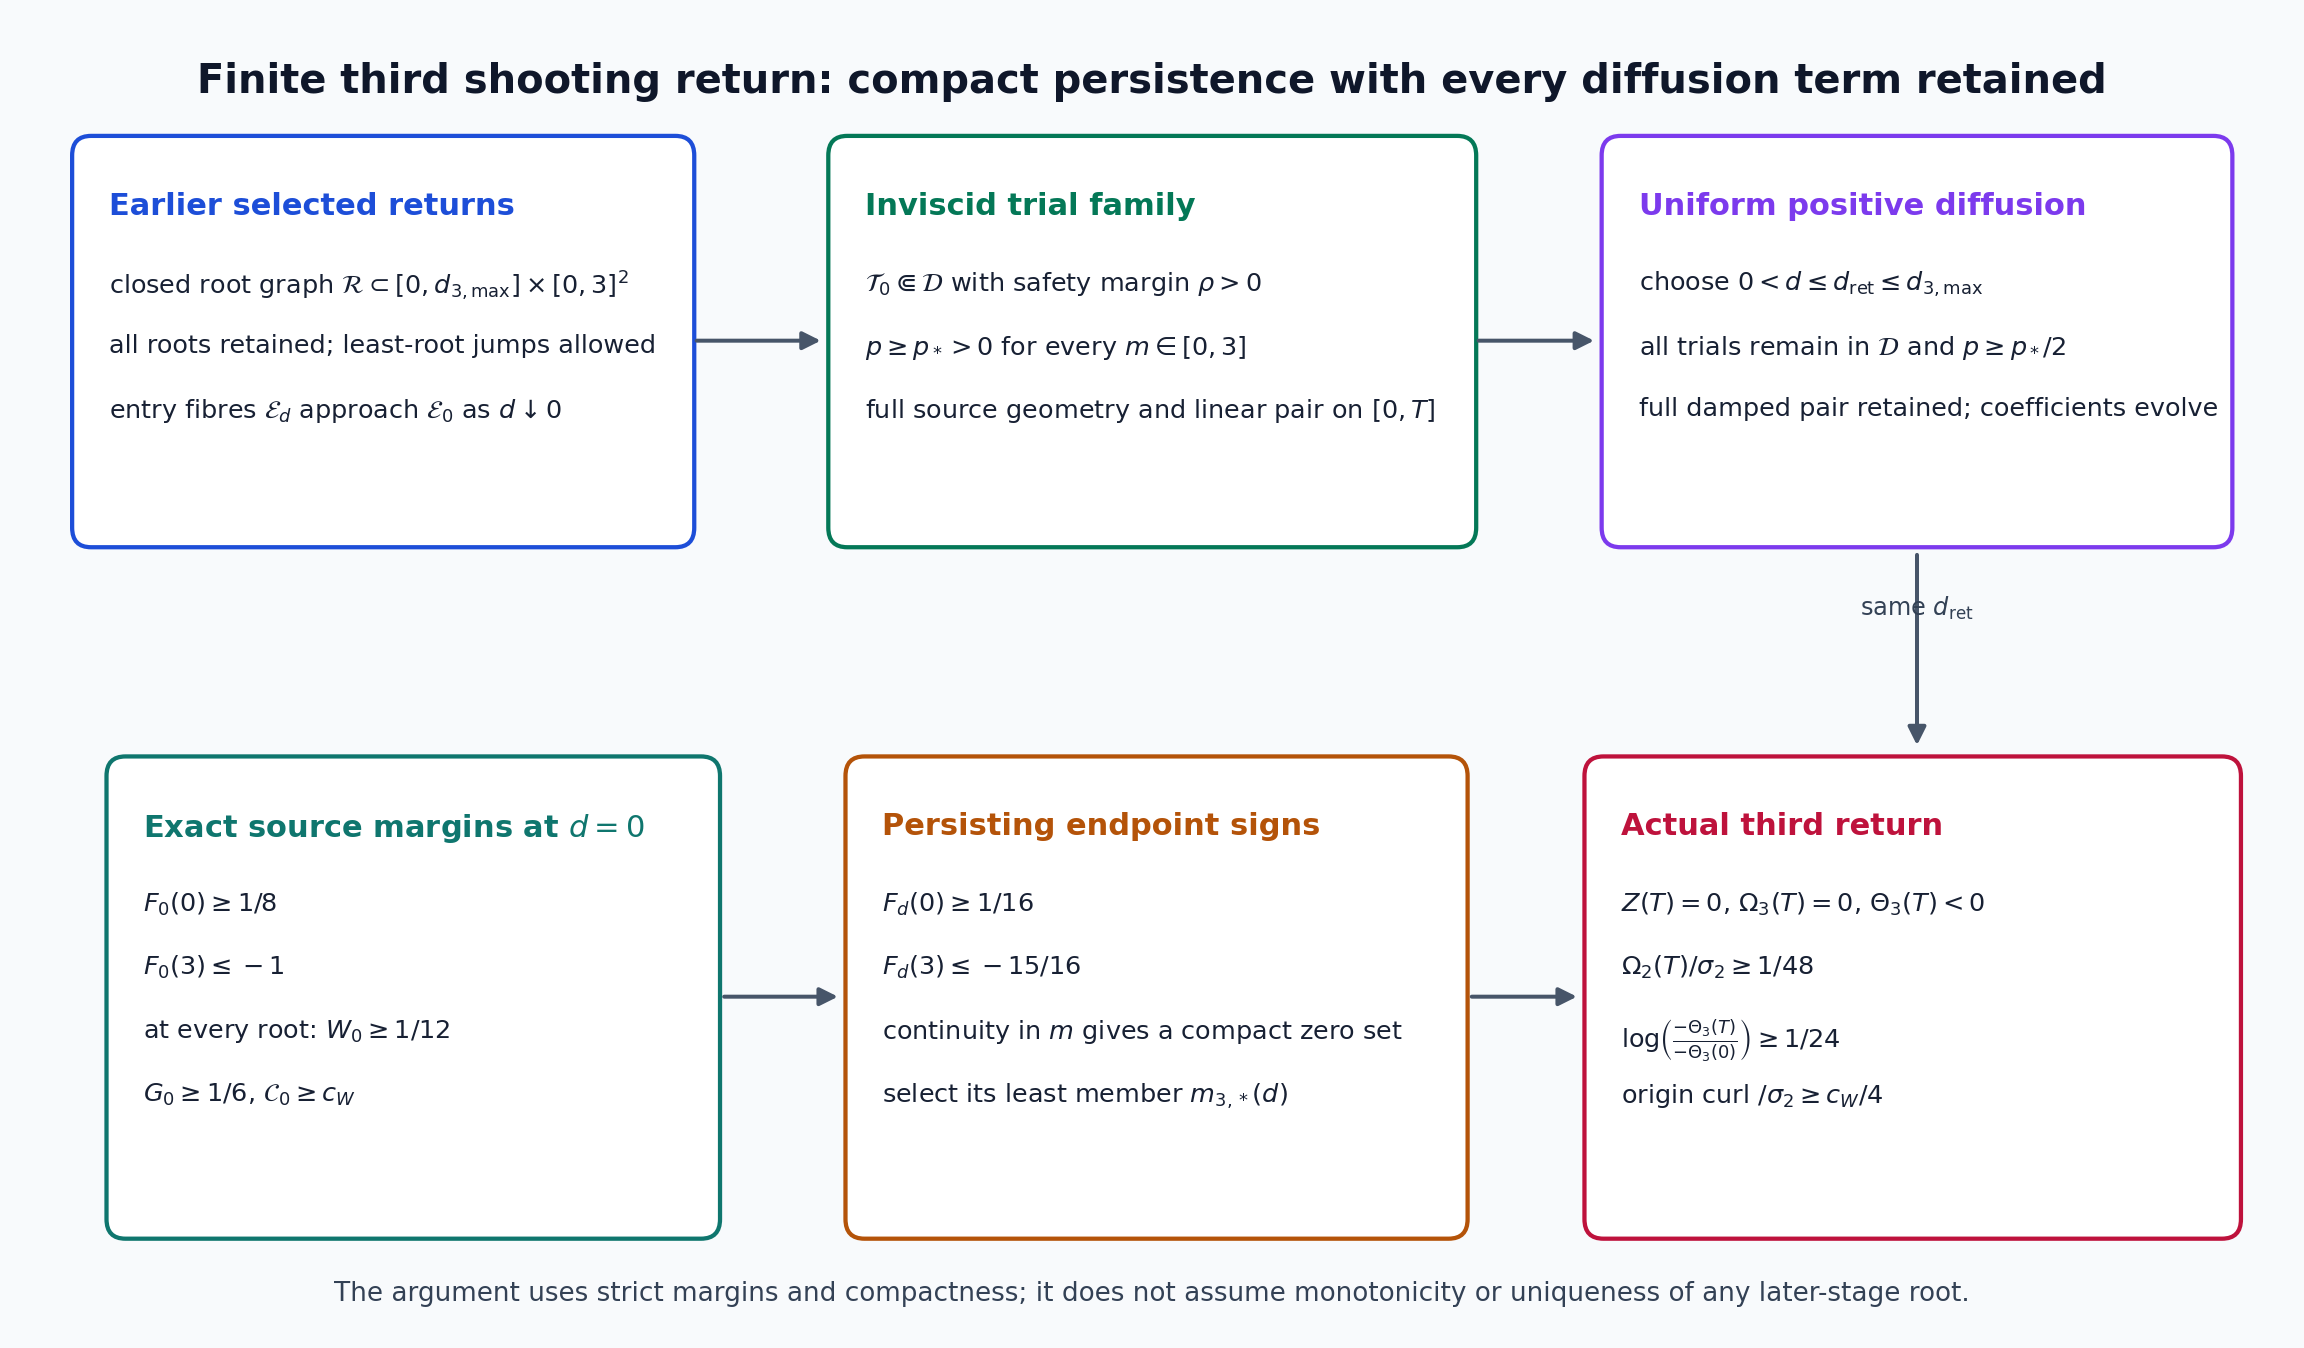
\includegraphics[width=0.96\linewidth]{third_return/figures/third_return_persistence.png}
 \caption{The exact finite persistence argument.  The inviscid entry and
 trial set has a compact trajectory image strictly inside the smooth
 component domain.  The closed earlier-root graph and uniform ODE
 continuation keep the positive-diffusion family in that interior.  The
 source endpoint margins persist, forcing a third endpoint zero and the
 displayed return bounds.  No monotonicity of the shooting map is used.}
 \label{trc:fig:persistence}
\end{figure}
